\documentclass{beamer}
\usetheme{Boadilla}


\usepackage{beamerthemesplit}
\usepackage[latin2]{inputenc}
\usepackage{colortbl}
\usepackage{hhline}
\usepackage{ae,aecompl,amsfonts}
\usepackage{fancyhdr}
\usepackage{hyperref}
\usepackage{verbatim}
\usepackage{array}
\usepackage{pstricks}
\usepackage{listings}
\usepackage{multirow}
\usepackage{wrapfig}

\newcommand{\listing}[2]{\begin{center}\parbox[b]{16cm}{\small\verbatiminput{#1}\normalsize\centering\mbox{Listing #2: Zawarto�� pliku #1}}\vskip 5mm\end{center}}
\newcommand{\HRule}{\rule{\linewidth}{0.5mm}}

\def\hilite<#1>{%
  				\temporal<#1>{\color{gray}}{\color{blue}}%
              				 {\color{blue!25}}}

\title[Haplotype frequency estimation\dots]{Heuristics for haplotype frequency estimation\\ with a large number of analyzed loci}
\author{Micha� Nowotka\inst{1} \and Robert Nowak\inst{2}}
\institute[Nowotka and Nowak]{
  
\includegraphics[width=0.12\textwidth]{images/logo}\\ \smallskip
  $^{1}$The Institute of Computer Science, Warsaw University of Technology
  \and
  $^{2}$The Institute of Electronic Systems, Warsaw University of Technology
}
\date{\today}

\begin{document}

\frame{\titlepage}

\section[Agenda]{}
\frame{\tableofcontents}

\section{Theory}
  	\subsection{Defining the problem}

		\frame[plain]
			{
  				\frametitle{Polymorphism}

					\begin{wrapfigure}{l}{0.35\textwidth}
						\centering
						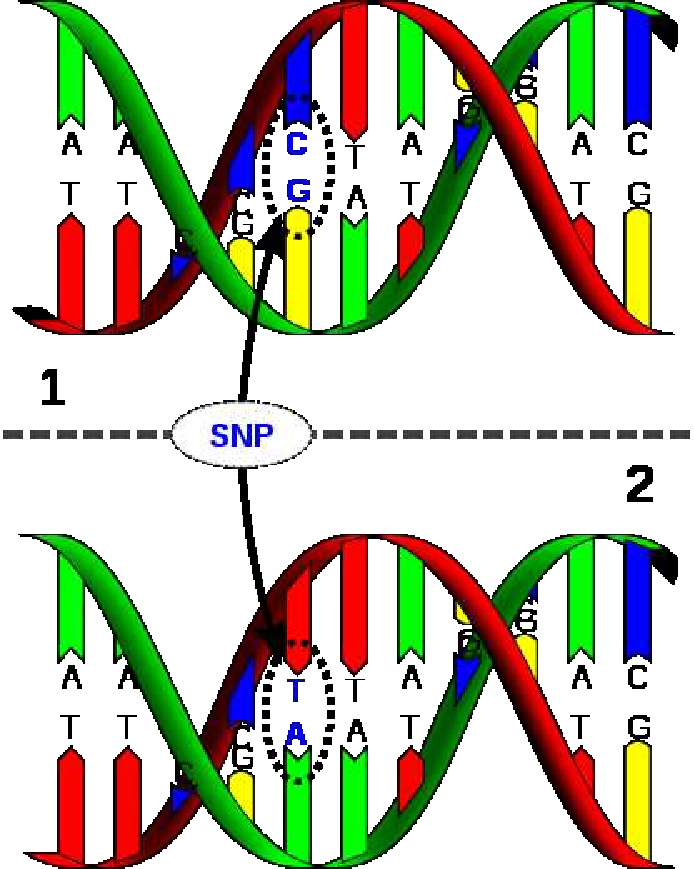
\includegraphics[width=0.23\textwidth]{images/SNP}
						\caption{A Single Nucleotide Polymorphism.}
					\end{wrapfigure}
					$\bullet$ \textbf{Polimorfism} -- occurrence of two or more alleles at the same single locus. \\ \medskip
					$\bullet$ \textbf{Genotype}~--~combination~of~alleles~the individual carries. \\ \medskip
					$\bullet$ \textbf{Haplotype} -- a~combination~of~alleles~at adjacent loci on the~chromosome~that~are transmitted together.

  			}

		\frame[plain]
			{
  				\frametitle{The problem}

					\begin{wrapfigure}{l}{0.43\textwidth}
						\centering
						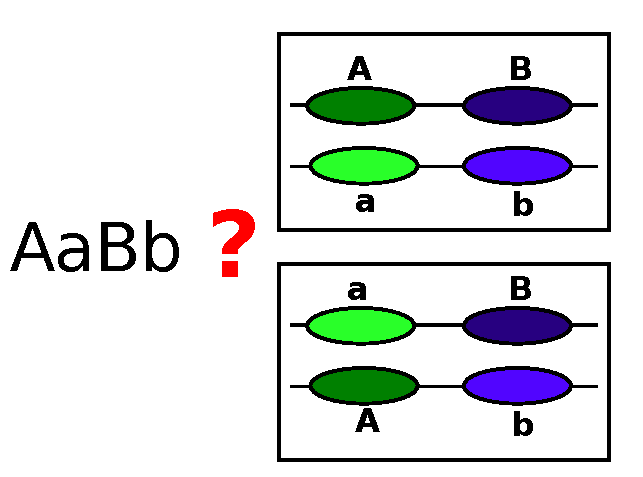
\includegraphics[width=0.43\textwidth]{images/poli}
						\caption{\small{Inferring haplotypes from genotypes}}
					\end{wrapfigure}
					$\bullet$~Determining~haplotypes~with~laboratory methods~is~expensive~and time-consuming. \\ \medskip
					$\bullet$ In~contrast,~there~are~many cost-effective~techniques~for~determining genotypes. \\ \medskip
					$\bullet$ In general, it could be impossible to inferre haplotypes from genotype data.

                    \begin{figure}
                      \begin{center}
					  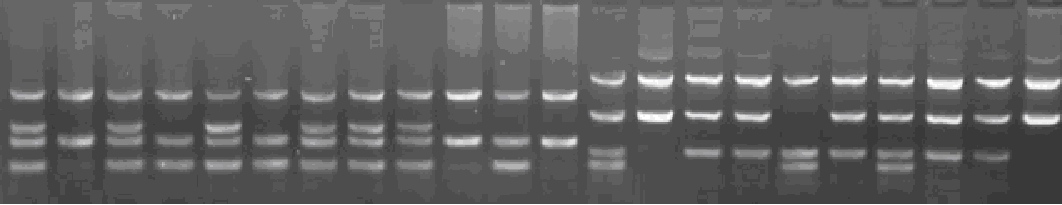
\includegraphics[width=\textwidth]{images/polimorfizmKIR}
					  \caption{\small{Determining genotype experiment results}}
                      \end{center}
                    \end{figure}



  			}

	  	\frame[plain]
			{
  				\frametitle{Null allele}

				\begin{figure}[h!]
					\centering
					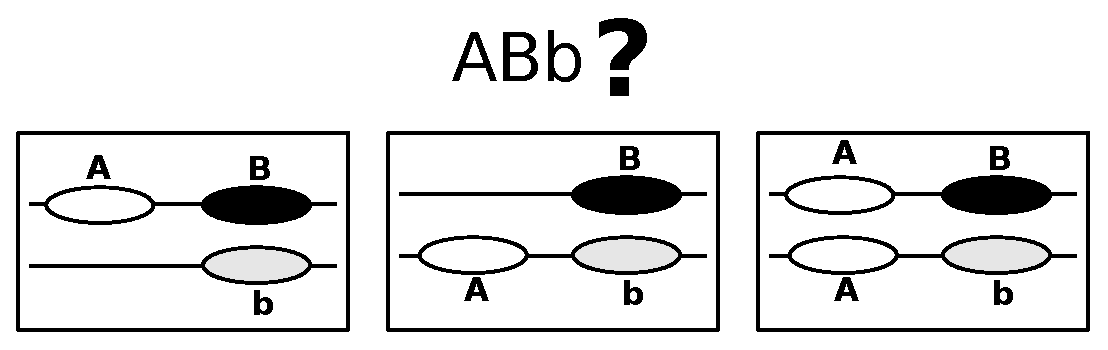
\includegraphics[width=0.8\textwidth]{images/null}
					\caption{\small{Inferring haplotypes from genotypes}}
				\end{figure}
  				\begin{alertblock}{Definition 4. Null allele}
                			A null allele is a copy of a gene that completely lacks that gene's normal function.
                			This can be the result of the complete absence of the gene product at the molecular level, or the expression of a non-functional gene product.
            			\end{alertblock}
  			}


  		\frame[plain]
			{
  				\frametitle{Different strategies for inferring haplotypes}

  				There are many different approaches to phasing problem:

  				\begin{itemize}
  					\item Pure parsimony
  					\item Hidden Markov Model and other Bayesian approaches
					\item Maximum-likelihood estimates
  				\end{itemize}

  				{
 				 \begin{block}{Definition 3. -- number of haplotype resolutions}

  					$$r_{j} = 2^{s_{j}-1}$$

  					where:
  					\begin{description}
  					   \item[$s_{j}$] --  number of observed loci.
  					\end{description}

  				\end{block}

  				\begin{alertblock}{Complexity problem}
				    The number of haplotype resolutions grows exponentially with $s_{j}$.
				\end{alertblock}
				}


  			}
  	\subsection{Solution}
		\frame[plain]
			{
				\frametitle{Idea of short overlapping windows}

				\begin{block}{Problem}
					Every algorithm emploing full space search would operate with $O(c^{n})$ complexity.
					This is why it cannot be directly applied to phasing long genotypes.
				\end{block}

				\begin{block}{Solution}
					Genotypes can be divided into shorter pieces that overlap.

					\begin{itemize}
						\item Piece length is fixed, so is computation time.
						\item Phasing n pieces has now $O(n)$ complexity.
						\item Multiple pieces can be phased in parrallel.
						\item If phasing algorithm is convergent total error should not be large.
					\end{itemize}
				\end{block}

			}

	  \frame[plain]
			{
				\frametitle{Short overlapping windows}
				   \begin{center}
  				   	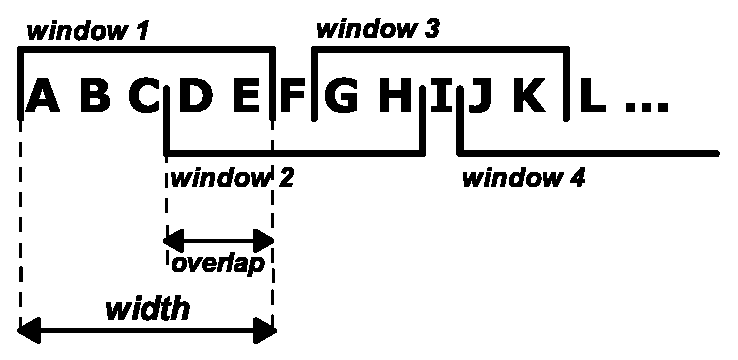
\includegraphics[width=0.45\textwidth]{images/window}
  					\end{center}

  					\begin{block}{Question}
  						What are the error and execution time as a function of \textbf{width} i \textbf{overlap} parameters?
  					\end{block}
			}

          	\frame[plain]
		   	{
            			\frametitle{Expectation Maximization algorithm}

            			\begin{itemize}
					\item Convergent
					\item Maximum likelihood
					\item May converge to a local maximum of the observed data
				\end{itemize}

             \begin{block}{Having:}
             	$$P(S|g_{1}, g_{2}, \dots, g_{G})$$
             \end{block}

             \begin{block}{We look for:}
             	$$\operatorname*{arg\,max}_{h_{1}, h_{2},\dots, h_{H}} P(S|h_{1}, h_{2},\dots, h_{H})$$
             \end{block}

             \begin{block}{Question:}
             	How to express $g$ in terms of $h$ ?
             \end{block}

         		}

          \frame[plain]
		   {
            \frametitle{Hardy-Weinberg Equilibrium}

            States that both allele and genotype frequencies in a population remain constant.

            \begin{block}{HWE (\textit{Hardy-Weinberg Equilibrium})}
            $$g_{j} = \sum_{i=0}^{r_{j}} z_{mn}$$ where
            	\[z_{mn} = \left\{
						\begin{array}{l l}
  							h_{m}^2 & \quad \mbox{for} m=n\\
  							2h_{m}h_{n} & \quad \mbox{for} m\neq n\\
						\end{array} \right. \]

            \end{block}

            \begin{alertblock}{Assuptions}
            	Lack of disturbing influences suich as non-random mating, mutations, selection, limited population size, random genetic drift, gene flow etc.
            \end{alertblock}
         }

	\subsection{Results}

		\frame[plain]
			{
				\frametitle{window-based approach -- results}

				\begin{center}
					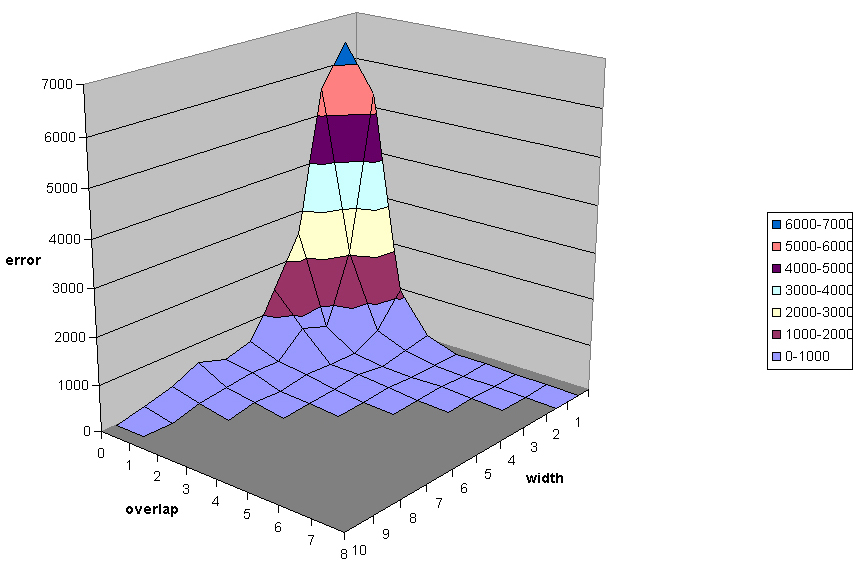
\includegraphics[width=0.75\textwidth]{images/error}
  				\end{center}
  			}

		\frame[plain]
			{
			  	\frametitle{window-based approach -- results}

 				\begin{center}
  				   	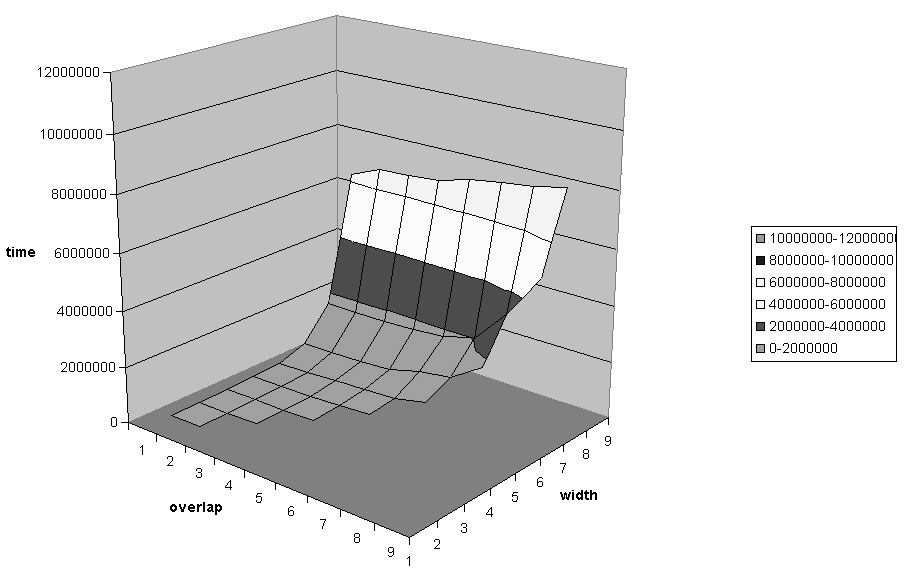
\includegraphics[width=0.75\textwidth]{images/czas}
  				\end{center}

			}

\section{Implementation}

		\frame[plain]
			{
				\frametitle{Application architecture}

				\begin{center}
					\includegraphics[width=0.47\textwidth]{images/scheme}
				\end{center}
			}


  	  	\frame[plain]
			{
  				\frametitle{Bibliography}
\begin{itemize}
\item F. Dellaert. The expectation maximization algorithm. Georgia Institute of Technology, Technical
Report Number GIT-GVU-02-20, 2002.

\item A. Gusev, I.I. Mandoiu, and B. Pasaniuc. Highly scalable genotype phasing by entropy minimization.
IEEE/ACM Transactions on Computational Biology and Bioinformatics (TCBB), 5(2):252?261,
2008.

\item R.M. Nowak and R. Ploski. NullHap -- a versatile application to estimate haplotype frequencies from
unphased genotypes in the presence of null alleles. BMC bioinformatics, 9(1):330, 2008.

\item P. Rastas, M. Koivisto, H. Mannila, and E. Ukkonen. A hidden Markov technique for haplotype
reconstruction. Lecture Notes in Computer Science, 3692:140, 2005.

\end{itemize}
  			}

  	  	\frame[plain]
			{

  				\begin{center}
  					\huge{\textbf{\textit{Thank you for your attention.}}}
  				\end{center}

  			}


\end{document}
